\section{Robot 4}

	\begin{figure}[h]
	\centering
	\subfloat[Figura de Matlab Robot 4.]{%
		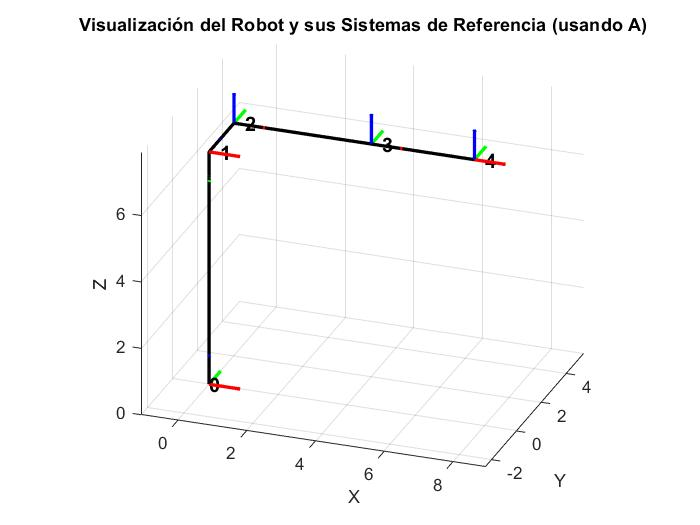
\includegraphics[width=0.5\textwidth]{ROBOT4MATLAB.jpg}%
		
	}
	\hspace{0.5cm} % Espacio entre imágenes (ajusta el valor si es necesario)
	\subfloat[Diagrama de lineas Robot 4.]{%
		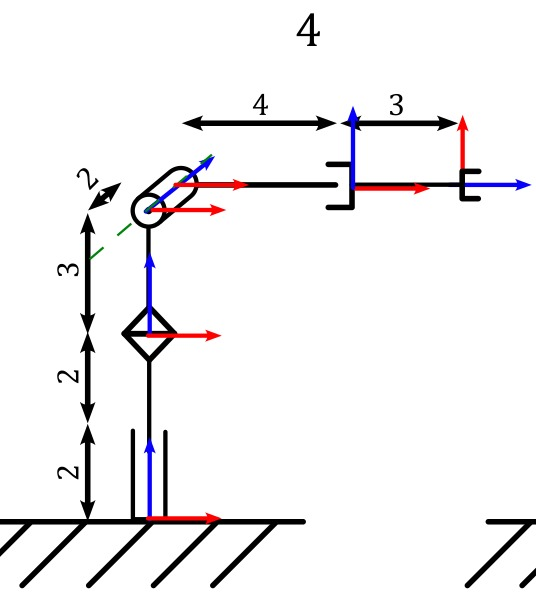
\includegraphics[width=0.35\textwidth]{DIAGRAMAROBOT4.jpeg}%
		
	}
	\caption{Ejercicio 4 de Denavit Hartenberg.}
	
\end{figure}
\vspace{8cm}